\newpage
\chapter{IMPLEMENTATION}\label{chapter_implementation}

All the algorithms of purposed handwriting recognition system are implemented in MATLAB \textregistered version 7.13.0.564 (R2011b). MATLAB is installed on a Intel(R) Core(TM)2 Duo CPU T6500 @ 2.10GHz processor. The Computer has total main memory of 2 Gigabyte and 32-bit Microsoft Windows 7 Ultimate operating system installed in it.

\section{MATLAB}
The name MATLAB stands for MATrix LABoratory. MATLAB is high-level technical computing language having high-performance computation. MATLAB started life in the 1970s as a user-friendly interface. It integrates computation, visualization, and programming in an easy-to-use environment where problems and solutions are expressed in familiar mathematical notation. MATLAB has very wide range of applications and can now be used as a very simple and transparent programming language where each line of code looks very much like the mathematical statement it is designed to implement. Typical uses of the MATLAB are given below.

\begin{itemize}
\itemsep0em 
\item Mathematical and scientific computation.
\item Algorithm development.
\item Application development, including Graphical User Interface building.
\item Data analysis, exploration and visualization.
\item Modelling, simulation and prototyping.
\item Graphics, in 2D and 3D, including colour, lighting and animation.
\end{itemize}


MATLAB is an interactive system whose basic data element is an array that does not require dimensioning. This allows solving many technical computing problems, especially those with matrix and vector formulations, in a fraction of the time it would take to write a program in a scalar non-interactive language such as C or FORTRAN. In university environments, it is the standard instructional tool for introductory and advanced courses in mathematics, engineering and science. In industry, MATLAB is the tool of choice for high-productivity research, development and analysis.

The reason behind using MATLAB for my research work experimentation is its wide variety and flexible toolboxes. Toolboxes are comprehensive collections of MATLAB functions (M-files) that extend the MATLAB environment to solve particular classes of problems. In this research work, mainly image processing toolbox and neural network toolbox are used along with other basis functionality of the MATLAB.

\section{Image Processing Toolbox}
\ac{ipt} is very rich MATLAB toolbox for working with images. It includes many powerful and very efficient image processing functions. It provides a comprehensive set of standard algorithms and graphical tools for image processing, analysis, visualization and algorithm development. We can use \ac{ipt} to perform complex image processing tasks like image enhancement, image deblurring, feature detection, noise reduction, image segmentation, geometric transformations, image registration, etc. Many toolbox functions are multithreaded to take advantage of multicore and multiprocessor computers.\par
Here, \ac{ipt} is used for image preprocessing techniques like noise removal, segmentation, skeletonization, etc. and for some feature extraction techniques (eg. euler number). It is also used for visualizing and analysing the results of image preprocessing and feature extraction steps.


\section{Neural Network Toolbox}
\ac{nnt} provides tools for designing, implementing, visualizing, and simulating neural networks. Neural networks are composed of simple elements operating in parallel. These elements are inspired by biological nervous systems. As in nature, the network function is determined largely by the connections between elements. We can train a neural network to perform a particular function by adjusting the values of the connections between elements. Neural networks are used for applications where formal analysis would be difficult or impossible, such as pattern recognition, identification, classification, speech, vision and control systems. Neural Network Toolbox supports feedforward networks, radial basis networks, dynamic networks, self-organizing maps, and other proven network paradigms. \ac{nnt} provides very customizable neural network functions which we can adjust according to our need. A typical neural network training contains following steps:
\begin{enumerate}
\itemsep0em 
\item Loading data source.
\item Selecting attributes required.
\item Decide training, validation, and testing data.
\item Data manipulations and Target generation.
\item Neural Network creation and initialisation.
\item Network Training and Testing.
\item Performance evaluation.
\end{enumerate}
In this research, \ac{nnt} is used for multilayer feedforward backpropagation network and radial basis function network training algorithms.

\addtocontents{toc}{\protect\setcounter{tocdepth}{1}}
\section{Feature Vector Creation} \label{section_feature_vector_creation}

%\addtocontents{toc}{\protect\setcounter{tocdepth}{1}}
%\subsection{This subsection is numbered but not shown in the toc}
%\addtocontents{toc}{\protect\setcounter{tocdepth}{2}}

Global feature vector is created according to the algorithms described in the section \ref{section_feature_extraction_methodology}. Let us consider image shown in figure \ref{figure_ka}. The binary matrix of this skeletonized image is given in figure \ref{figure_binary_matrix_of_ka}. 

\begin{figure}[ht]
\begin{minipage}[b]{0.5\linewidth}% skeletonized image 'ka'
\centering
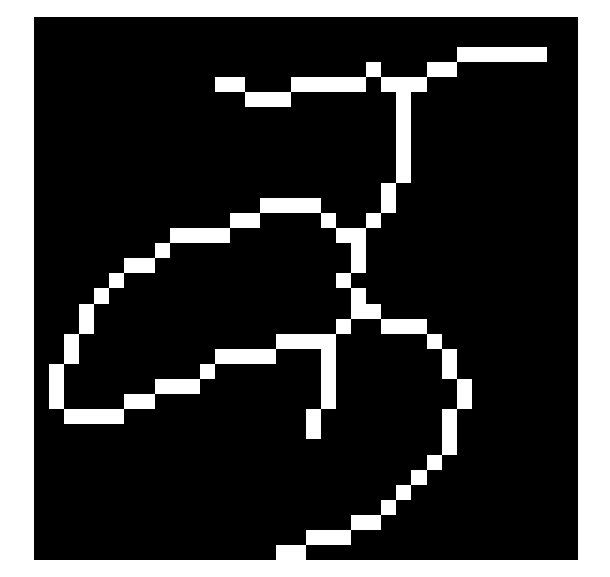
\includegraphics[scale=0.35]{figures/ka_features/ka.eps}
\caption{Nepali consonant letter 'ka'.}
\label{figure_ka}
\end{minipage}
\hspace{0.5cm}
\begin{minipage}[b]{0.5\linewidth}% image 'ka' in binary matrix form
\centering
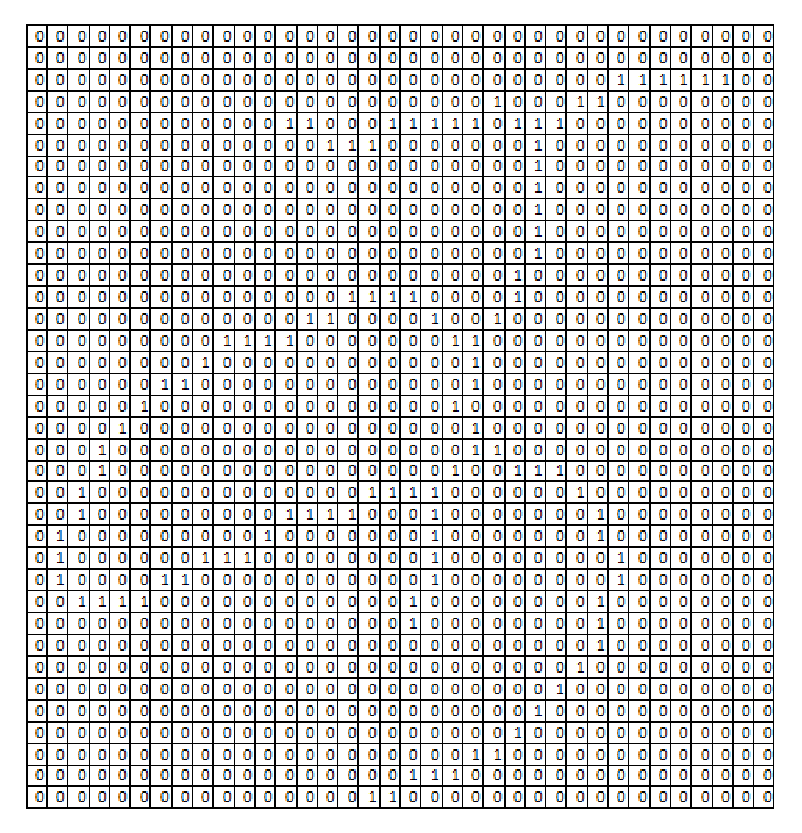
\includegraphics[scale=0.30]{figures/ka_features/ka_binary_matrix.eps}
\caption{Letter 'ka' as binary matrix.}
\label{figure_binary_matrix_of_ka}
\end{minipage}
\end{figure}

\subsection{Directional Feature Vector}
For the directional feature extraction, image is zoned into 3x3 sub-images. Figure \ref{figure_ka_zoned} shows zoned images of image given in the figure \ref{figure_ka}.

\begin{figure}[h]
\centering
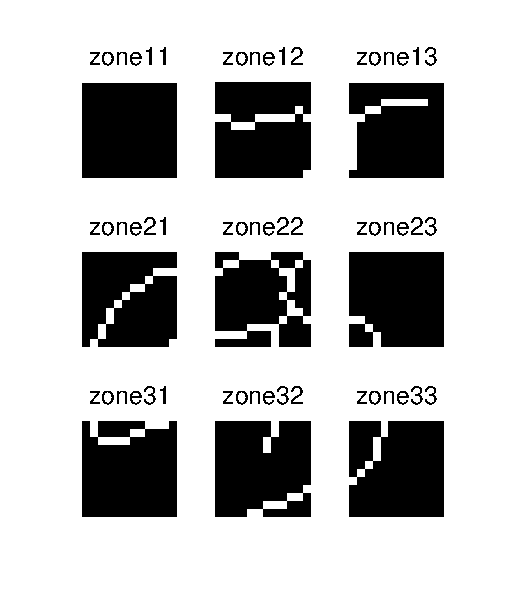
\includegraphics[scale =1]{figures/ka_features/ka_zoned.eps}
\caption{Zoned images}
\label{figure_ka_zoned}
\end{figure}

Normalized feature vectors corresponding to each zone are given in Table 5.1. %\ref{table_directional_feature_vectors}.

\captionsetup[table]{list=no}
\begin{table}[h]
\label{table_directional_feature_vectors}
\centering
\begin{tabular}{|c|c|}
\hline  zone11 feature vector & [-1,-1,-1,-1,-1,-1,-1,-1,-1] \\ 
\hline  zone12 feature vector&  [0.80,1,1,1,0.85,0,0,0,1]\\ 
\hline  zone13 feature vector&  [0.80,1,1,1,0.85,0,0,0,1]\\ 
\hline  zone21 feature vector&  [1,1,0.80,1,0,0,0.86,0,1]\\ 
\hline  zone22 feature vector&  [0.60,0.80,0.80,0.80,0.63,0.03,0.06,0.03,0.40]\\ 
\hline  zone23 feature vector&  [1,1,1,0.80,0,0,0,0.80,1]\\ 
\hline  zone31 feature vector&  [0.80,1,1,1,0.90,0,0,0,1]\\ 
\hline  zone32 feature vector&  [0.80,0.80,1,1,0.58,0.25,0,0,1]\\ 
\hline  zone33 feature vector&  [1,1,0.80,1,0,0,0.87,0,1]\\ 
\hline 
\end{tabular}
\caption{Directional feature vectors corresponding to figure \ref{figure_ka_zoned}.}
\end{table}
\captionsetup[table]{list=yes}

\subsection{Moment Invariant Feature Vector}
Moment invariant features are extracted from whole character image. It implements the algorithm given in section \ref{section_moment_invariant_features}. Moment invariant features corresponding to figure \ref{figure_ka} are given below,
\begin{center}
[ 1.3937, 0.1858, 0.8792, 0.0024, 0.0001, 0.0009, -0.0001]
\end{center}

\subsection{Euler Number Feature Vector}
There is a single entry for Euler number in global feature vector. An Euler number corresponding to figure \ref{figure_ka} is 0.

\subsection{Normalized Area of Character Skeleton Feature Vector}
There is a single entry for normalized area of character image in global feature vector. Normalized area corresponding to figure \ref{figure_ka} is 0.0841. Normalized area is calculated by following formula.\par
$$normalized\_area=1-\frac{area}{image\_size}$$

\subsection{Centroid Feature Vector}
Centroid is also extracted from whole character image. There are two entries for centroid in global feature vector. Normalized centroid corresponds to figure \ref{figure_ka} is given below,
% $$ [18.5413, 18.1743]$$
$$ [0.9857, 0.9860]$$

\subsection{Eccentricity Feature Vector}
There is single entry in global feature vector for eccentricity. Eccentricity corresponds to figure \ref{figure_ka} is 0.6870.

\subsection{Global Feature Vector}
\addtocontents{toc}{\protect\setcounter{tocdepth}{4}}
Global feature vector is created by appending all above feature vectors to a single feature vector. There is 93 dimensional global feature vector for each character images. The global feature corresponds to figure \ref{figure_ka} is given below,\par

input\_vector=[ -1, -1, -1, -1, -1, -1, -1, -1, -1, 0.80, 1, 1, 1, 0.85, 0, 0, 0, 1, 0.80, 1, 1, 1, 0.87, 0, 0, 0, 1, 1, 1, 0.80, 1, 0, 0, 0.86, 0, 1, 0.60, 0.80, 0.80, 0.80, 0.63, 0.03, 0.07, 0.03, 0.40, 1, 1, 1, 0.80, 0, 0, 0, 0.80, 1, 0.80, 1, 1, 1, 0.90, 0, 0, 0	1, 0.80, 0.80, 1, 1, 0.58, 0.25, 0, 0, 1, 1, 1, 0.80, 1, 0, 0, 0.87, 0, 1, 0.999, 0.999, 0.999, 0.999, 0.999, 0.999, 1.00, 0, 0.08, 0.98, 0.98, 0.69].

To create target vector corresponding to above global feature vector, we create a vector with dimensionality equal to output classes. For figure \ref{figure_ka}, since it belongs to Nepali consonant class, we have 36 dimension target vector with first entry equal to 1 and all other entries equal to 0. So, the target vector corresponds to figure \ref{figure_ka} is given by,\par
target\_vector=[1, 0, 0, 0, 0, 0, 0, 0, 0, 0, 0, 0, 0, 0, 0, 0, 0, 0, 0, 0, 0, 0, 0, 0, 0, 0, 0, 0, 0, 0, 0, 0, 0, 0, 0, 0].

Now, above feature vector along with corresponding target vector is ready to feed into neural network for training and testing. Training is done in supervised manner with two neural network algorithms, \ac{mlp} and \ac{rbf} networks.



% \section{Neural Network Training and Testing}
